\chapter{Fast Predecessor Search in Small Set}
\label{chap:predecessor}

In this chapter, the problem of predecessor search in small sets is addressed. This problem was previously perceived to be impractical due to the lack of hardware to support some of the theoretical claims. Using SIMD instructions, a practical and efficient implementation of constant time predecessor search in integer sets is provided, leveraging Single-Instruction-Multiple-Data (SIMD) instructions. Experimental evaluations demonstrate that these data structures can be implemented and are useful in applications such as B-Trees and super-scalar search and sorting.

The novel contributions of this chapter are: (i) a practical implementation of Ajtai's constant-time predecessor search using pre-computed lookup tables with SIMD instructions --- to the best of available knowledge, the first such practical implementation; (ii) an improved variant of Fredman's method that exploits XOR-minimisation to maximise the longest common prefix, yielding faster query times with no additional memory overhead; (iii) an analysis of significant bit positions across synthetic and real-world datasets; and (iv) comprehensive empirical comparisons demonstrating 3.5--5.2$\times$ speedups over linear search for small static sets.
\section{Introduction}
\label{sec:Introduction}
Predecessor search is amongst the most fundamental algorithmic problem in computer science \cite{Degermark_1997}. An important sub-case is that of searching a small static set of integer keys.  On the word RAM with word size $w$ bits, ``small'' is usually taken to mean $w^{O(1)}$.  A number of papers have explored this problem \cite{AJTAI1984217,FREDMAN1993424, Patrascu_2014} and have proposed $O(1)$-time and linear-space solutions to this problem, improving upon comparison-based approaches that would take time logarithmic in the number of keys ($O(\log w)$ time in this case). These solutions are either described in the \emph{cell probe} model \cite{AJTAI1984217}, where the algorithm is only charged for the reads and writes it makes to memory (and can compute arbitrary functions on data in registers for free), or make complicated, and ingenious, \textit{bit-parallel} tricks to simulate SIMD operation on several items packed into $w$-bit words. Their complexity has hitherto led to these algorithms being viewed as impractical.\par
In recent years, the range of instructions built into CPUs has increased tremendously, and this leads us to re-examine the practicality of the above approaches. In addition, all of the existing approaches broadly use a \textit{blind trie} search (see below for a description). The  practicality of these approaches depends heavily on the number of \emph{significant bit positions} in the input keys (see below, but very roughly, considering the keys as bit-strings, we place them in a trie, and look at which positions are in fact needed to navigate to a leaf).  In a set of $k$ keys, the number of 
 significant bit positions in the worst case is $k-1$ and the above algorithms proceed with this assumption.  However, in the best case the number of significant bit positions only needs to be $O(\log k)$, and practical applications may or may not have many significant bit positions.  For example, in one application we consider, namely maintaining a dynamic bit-vector \cite{Prezza17}, the keys are the prefix sums of the sizes of the sub-trees of a given node; these behave much better than the worst case. Based upon these insights, we implement and empirically evaluate predecessor search algorithms based on \cite{AJTAI1984217} and \cite{FREDMAN1993424}, and show clear improvements over comparison-based methods.\par

\section{Preliminaries} \label{sec:preliminaries}
Let $X$ be a set of $n$ (where $n$ is $|X|$) positive integers drawn from universe $U$. The following operations are defined for any $x \in X$:
\begin{itemize}
    \item \textit{access(i):} returns the elements $X[i]$ for $0 \leq i < n$.
    \item \textit{predecessor(x):} returns the maximum element $y \in X$ such that $y \leq x$.
    \item \textit{member(x):} returns \textit{true} if $x \in X$ and \textit{false} otherwise.
\end{itemize}
Under the \textit{word-RAM} model, arithmetic and logical operations are expected to be performed in $O(1)$ time. There are some additional operations that are expected to also run in \textit{constant} time, such as counting the number of trailing/leading bits in $s_i$ and number of set bits in $s_i$. The most common theoretical approach previously was to use a pre-computed look-up table, but with advancements in \textit{built-in} instructions~\cite{AMD64_2020, ARM_A64_2018, Intel_IA32_2016}, this can now be supported practically in $O(1)$.
\par
\subsection{Advanced Bit Manipulation Instructions}
%\input{lipics-v2019-authors/Example1}
An operation $lcp(x, y)$ is defined that for two integers $x$ and $y$ computes the bit position where $x$ and $y$ share the longest common prefix. Built-in functions and compiler intrinsics are used to achieve this in constant time by computing the $exclusive-or$ between $x$ and $y$, and then counting the number of leading zeros using LZCNT\footnote{https://software.intel.com/sites/landingpage/IntrinsicsGuide/} to determine the longest common prefix.
\begin{table}[ht]
    \centering
    \begin{minipage}[t]{1\textwidth}
        \centering
        \begin{algorithm}[H]
            \caption{LCP(c, y)}
            \begin{algorithmic}[1]
                \STATE z =: x $xor$ y
                \RETURN \textit{lzcnt(z)}.
            \end{algorithmic}
        \end{algorithm}
    \end{minipage}%
\end{table}

\subsection{Blind Search} A Patricia trie $P(S)$ otherwise called a compact trie is derived from a normal trie by replacing each sub-string on an edge with its first character (also called a \textit{branching-character}), and merging any only child with its parent. A $blind-search$ introduced by Ferragina \cite{Ferragina_Grossi_1999} looks for a given string $s$ in $S$ by comparing only the available branching characters. This search procedure ends at either of the following: (a) $s$ is exhausted and a leaf $v$ is reached; or (b) a mismatch happened when branching from a node $v$. Ferragina \cite{Ferragina_Grossi_1999} suggests that any leaf $u$ in the sub-tree of $v$ shares the \textit{longest common prefix} (LCP) with $s$. The value $l = LCP(s, S[u])$ indicates the bit position where $s$ should have branched out. With this new information and another blind search for $s$, the exact position of $s$ in $S$ can be computed. 
\begin{figure}[H]
\centering
\begin{forest}
for tree={circle, draw, l sep+=10pt, s sep+=10pt, inner sep=1.5pt, edge={-, thick}}
[0 
  [1, edge label={node[midway, left]{0}}
    [\textbf{0}, edge label={node[midway, left]{0}}] 
    [2, edge label={node[midway, right]{1}} 
      [\textbf{1}, edge label={node[midway, left]{0}}] 
      [\textbf{2}, edge label={node[midway, right]{1}}]
    , edge label={node[midway, right]{1}}]
  , edge label={node[midway, left]{0}}] 
  [2, edge label={node[midway, right]{1}}
    [5, edge label={node[midway, left]{0}} 
      [\textbf{3}, edge label={node[midway, left]{0}}] 
      [\textbf{4}, edge label={node[midway, right]{1}}]
    , edge label={node[midway, left]{0}}] 
    [\textbf{5}, edge label={node[midway, right]{1}}]
  , edge label={node[midway, right]{1}}]
]
\end{forest}
\caption{Blind trie for $S = \{ 7, 85, 102, 200, 205, 232 \}$ showing the significant bit positions in the internal nodes and significant bit positions on edges. The leaves hold the index $i$ of $S[i]$}
\end{figure}

\subsection{Significant Bit Positions}  A branching point is the index of the longest common prefix between two integers $x, y$. Given an input of $w$-bit integers $S$ of size $k = |S|$, the set of significant bit positions $B(S)$ is all the distinct bit positions of $lcp(s_i, s_{i+1})$ for all $s_i \in S$ and $0 \leq i \leq {k-1}$. The upper bound on the number of significant bit positions for $k$ keys is $k$, while the lower bound is $\log k$. This is trivial to see that the upper bound is possible when all the keys have a different $lcp$, while on the lower bound side, we need at least $\log k$ bits to be able to uniquely identify $k$ elements.\par
\begin{lemma}
Given a set of sorted $w$-bits integers $S$ of length $k$, computing the $lcp$ between
consecutive adjacent elements in $S$ gives all the significant bit positions in $S$.
\end{lemma}\par
\textit{Proof:}
Two adjacent integers $(x, y) \in S$ share the longest common bits compared to any other combination of $(x, z) \in S$, which makes the lemma to hold trivially. If $(x, z)$ has an $lcp$ greater than $(x, y)$, then $z < y$, and that violates the sorting order of $S$.\par
\textbf{Example 1.}
\begin{itemize}
    \item Let $S = \{ 7, 85, 102, 200, 205, 232 \}$
    \item $k = 6$
    \item Set of significant bit positions is $B = \{ 0, 1, 2, 5 \} $ after removing duplicates.
    \item Mask generated from $B = 228$ which is $11100100$ in binary (with padding).
\end{itemize}

\subsection{Compressed Keys} Fredman et al.~\cite{FREDMAN1993424} proposed the idea of using compressed keys as part of their data structure that supports constant time predecessor search on $S$ with $k = w^{1/6}$. Given a key $x$, a compressed key $\hat{x}$ is a key containing only the bits of $x$ at significant bit positions (with some additional padded zeros). Key $\hat{x}$ is of length $b \leq k^3$. A set of compressed keys $\hat{S}$ contains the compressed keys from $S$. The use of compiler intrinsics to compress $x$ in constant time and be of length $b \leq |B|$ is proposed. First, a mask $m$ of length $k$ is created with the bits at index $i$ in $m$ set to $1$ if $i$ is a branching bit, and $0$ otherwise. Then \texttt{PEXT}\footnote{https://software.intel.com/sites/landingpage/IntrinsicsGuide/} is used to extract the bits at the positions specified by the mask.\par
\begin{table}[ht]
    \centering
    \begin{minipage}[t]{1\textwidth}
        \centering
        \begin{algorithm}[H]
            \caption{Compress(x, m)}
            \begin{algorithmic}[1]
                \RETURN \textit{$\_pext\_u64(x, m)$}.
            \end{algorithmic}
        \end{algorithm}
    \end{minipage}%
\end{table}

\textbf{Example 2.}
\begin{itemize}
    \item Let $S = \{ 7, 85, 102, 200, 205, 232 \} $
    \item The mask generated from significant bit positions of $S$ is $m = 228$
    \item $\hat{S} = \{ 1, 5, 7, 12, 13, 14 \}$
\end{itemize}

\subsection{Ajtai's Method}
Ajtai \cite{AJTAI1984217} presented a constant time data structure for searching in small integer set $S$. They build a Patricia trie $P(S)$ of the elements of $S$ represented as binary strings of length $\lceil \log u \rceil$ where $u$ is the universe of the set. Assuming that $P(S)$ fits into a machine word, they show that they can search for a given key $x$ in $P(S)$ and returns an index $i$ of the leaf matching $x$ in constant time. This is because of the assumption that operations on machine word takes $O(1)$ time. Then they computed $j = lcp(S[i], x)$, and complete the search by another operation that returns the rank of $x$ in $P(S)$ assuming $x$ branches out at $j$. All these operations are in constant time using RAM model. They concluded that \textit{"the algorithm is not very realistic as searching through a trie requires more than constant time in actuality"}.

\subsection{Fredman's Method}
Fredman \cite{FREDMAN1993424} improved on the above by introducing $rank$ on a set in constant time assuming all the elements of the set can fit in machine word $w$. To do predecessor search on $S$, they pre-process $S$ to extract all the significant bit positions (with extra irrelevant zeros) and store them in an array $B$, and then compressed $S$ by extracting only the significant bit positions in every element in $S$ and form another array of compressed keys $\hat{S}$. Assuming $\hat{S}$ also fits into a machine word, they can compute $rank(\hat{S}, i)$ in constant time. They argue that either $y = S[i]$ or $y = S[i+1]$ has the longest common prefix $j$ with $x$. If the compressed trie was used, then $i$ and $h = rank(B, i)$ determines the edge $(u, v)$ where $x$ should have branched out. The predecessor of $x$ is the largest key below $v$ if $x_j = 1$; otherwise, the successor is the smallest key below $v$. Using lookup tables to perform these operations, they showed that they can support this in constant time.

\subsection{SIMD and Builtin Instructions} SIMD instructions allow for parallel processing of $k$ data sets per instruction where $k$ is determined by the processor and $w$. SIMD registers come in various sizes of $128$-bits (in SSE) and $256$-bits (AVX/2), and the most recent but not widely available $512$-bit (AVX512) registers support larger data sets. The $256$-bit registers that come with AVX/2, which are widely available in most \textit{Intel processor} machines, are considered here.\par
\begin{table}[h]
    \centering
    \begin{tabularx}{\textwidth}{|l|c|c|X|}
    \hline
         \textbf{Instruction} & \textbf{Type} & \textbf{CPUID} & \textbf{Description} \\\hline
         $PEXT(a, b)$ & Builtin & BMI2 & Extracts and deposit bits from $a$ based on positions specified by mask $b$\\\hline
         $LZCNT(a)$ & Builtin & LZCNT & Count the number of leading zeros in $a$\\\hline
         $TZCNT(a)$ & Builtin & BMI1 & Count the number of trailing zeros in $a$\\\hline
         $\_mm256\_set1\_epi16(a)$ & SIMD & AVX & Broadcast $a$ as a 16-bit element to all elements of the 256-bits register\\\hline
         $\_mm256\_loadu\_si256(*a)$ & SIMD & AVX & Loads and read into a 256 register 256-bits of data specified by memory location $a$ \\\hline
         $\_mm256\_xor\_si256(a, b)$ & SIMD & AVX & Horizontally computes the bitwise XOR of 256-bits registers $a$ and $b$ \\\hline
         $\_mm256\_movemask\_epi16(a)$ & SIMD & Created & Creates mask from the most significant bit of each $16-bit$ element in 256-bits register $a$ \\\hline
         $\_mm256\_minpos\_epi16(a)$ & SIMD & Created & Horizontally computes the minimum amongst the packed 16-bits elements in 256-bits register $a$ \\\hline
    \end{tabularx}
    \caption{Instructions used and their descriptions}
    \label{tab:simd-instructions}
\end{table}
\par
Bit-manipulations have increasingly become important to fast data structures, with most approaches relying on some clever \textit{bit-hacks} and programming tricks~\cite{hilewitz_2008}. Both algorithms considered in this chapter are heavily reliant on bit-wise manipulation to perform their operations. This makes their approach complex and challenging. The Bit Manipulation Instructions (BMI) that are an extension of the x86 instruction set architecture and operate on general purpose registers are exploited. The instructions used can be largely grouped into the following categories:
\begin{itemize}
    \item \textit{Load and store}: this group of instructions loads and copies data from a continuous chunk of memory into a SIMD register. When the data to be read is from non-continuous memory locations, this slows down these operations as a separate $read$ operation will be needed for each location.
    \item \textit{Element-wise}: this group of instructions performs an operation on a specific data element within a single or multiple SIMD registers. These could include $shifting$ and $access$.
    \item \textit{Horizontal-wise}: these sets of instructions act across the elements of a SIMD register. It allows for operations to be performed on values stored within a register. For example, adding or multiplying two values within the same register and permutation of values within a register.
    \item \textit{Advanced BMIs}: these are bit manipulation instructions implemented as single instructions in $intel$ processors that were considered expensive before. These include $PDEP$ and $PEXT$.
\end{itemize}

\FloatBarrier
\section{Computing Significant Bit Positions} \label{branchingbits}
An experiment to compute the number of branching positions in various synthetic data sets is presented. The first dataset is aimed at generating the worst case number of significant bit positions, the second dataset generates uniformly distributed random numbers using the C++ STL random number generator\footnote{https://en.cppreference.com/w/cpp/numeric/random}, the third dataset is based on the sizes of B-tree nodes, and the last dataset is based on the B-tree splitter keys.\par
\textbf{Worst Case:} A potential worst-case input scenario that could generate the maximum possible significant bit positions is shown. To generate $k$ integers, a sequence $S$ of length $k$ is generated as powers of $2$ by setting $S[i] = 2^i$ for $0 < i < k$.
\par
\textbf{Example 3.}
\begin{itemize}
    \item Let $k = 6$ and word size $w = 5$ bits.
    \item Then $S = \{0, 2, 4, 8, 16, 32\} $
    \item The set of branching position $B = \{ 0, 1, 2, 3, 4, 5 \}$
\end{itemize}
\par
\subsection{Random Datasets} For the random dataset, the C++ Mersenne Twister pseudo-random generator engine\footnote{http://www.cplusplus.com/reference/random/mt19937/} is used to generate small sets of 64-bit integers. The resulting set is then sorted and the number of significant bit positions is computed.
\par
\subsection{B-Tree Sub-Tree Size Datasets} Given $k$, $b$ (the B-tree fan-out) is set equal to $k$, and $h$ (the height of the B-tree) is set to a random number. $S$ is initialised with an initial size of $n \leq k$ and each $S[i] = b^h$ for $0 \leq i \leq n$. Then $b^h$ random increments are made in $S$ with two conditions: (a) if $S[j] < 2b^h$, then $S[j] = S[j] + 1$ is set (b) else if $S[j] = 2b^h$, $S[j]$ is split into two by setting $S[j] = b^h$, shifting $S[j+q]$ to the right where $1 \leq q \leq n$, and finally setting $S[j+1] = b^h$, after which the increment continues. When the increments are finished, the first $k$ elements in $S$ are taken, and a prefix sum of their values forms the dataset.\par
The idea is to simulate B-tree sub-tree sizes of fan-out $b$ and height $h$. This means the size of the B-tree cannot be greater than $b^h$, and whenever an insertion leads a node $j$ to be greater than $b^h$, the node is split into two sub-trees.
\par
\subsection{B-Tree Splitter Keys Datasets} The splitter keys in a B-tree are the largest/smallest keys of the sub-trees. A B-tree sub-tree dataset $D$ of size $N$ where $N$ is large is created and its prefix sum is taken. Given $k$ as the size of the required input, $S[i] = D[i*k]$ is set for $0 \leq i < k$ to get the smallest splitter keys of the B-tree. Alternatively, $S[i] = D[i*(k+1)]$ can be set for $1 \leq i \leq k$ to get the largest splitter keys of the B-tree.\par
\begin{figure}[H]
    \centering
    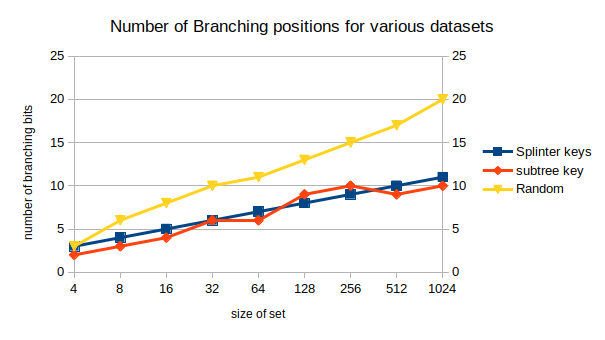
\includegraphics[width=17cm,keepaspectratio]{images/NBBTest.png}
    \caption{Number of significant bit positions for various datasets}
    \label{fig:number_of_branching_bits}
    
\end{figure}
\section{Optimisations} A technique to reduce the number of significant bit positions in a set $S$ is proposed. The hypothesis is that if the set $S$ is $shifted$ to $S+x$ by making $S[i] = S[i] + x$ for all $1 \leq i \leq k$, where $x$ is a random integer, the significant bit positions of some values of $S$ will be shifted, which will in turn increase the number of duplicates in $B$ and thus reduce the number of significant bit positions. Random inputs of various sizes were generated and each input was shifted by values $i$ where $1 \leq i \leq 2^{16}$. The maximum, minimum and average number of significant bit positions for each of the data sets were computed and are reported below. The baseline is the number of significant bit positions of the generated input before the shifting is started.\par
\begin{table}[H]
\centering
\begin{tabular}{|l|c|c|c|c|c|c|c|c|c|c|}
\hline
\textbf{Metric/Input Size} & \textbf{4} & \textbf{8} & \textbf{16} & \textbf{32} & \textbf{64} & \textbf{128} & \textbf{256} & \textbf{512} & \textbf{1024} & \textbf{2048} \\ \hline
Baseline  & 3  & 5  & 6  & 9  & 9  & 11 & 12 & 13 & 13 & 15 \\ \hline
Minimum       & 2  & 3  & 4  & 4  & 6  & 7  & 8  & 9  & 10 & 12 \\ \hline
Average   & 3  & 5  & 7  & 8  & 9  & 10 & 11 & 12 & 14 & 15 \\ \hline
Maximum       & 3  & 7  & 11 & 12 & 14 & 14 & 15 & 16 & 19 & 19 \\ \hline
\end{tabular}
\caption{Result of shifting input of various array sizes by values between $0 - 12000$.}
\label{table:reducingnbb}
\end{table}
\par
From Table~\ref{table:reducingnbb}, some improvements in the number of significant bit positions at certain shift values can be seen, which can reduce space usage of Ajtai~\cite{AJTAI1984217} lookup tables. This is intended to be explored further as part of future work. Questions such as the following are intended to be answered: \textit{what value of $i$ should $S$ be shifted by to reduce the number of significant bit positions below the baseline?}
\FloatBarrier
\section{Implementations Using Built-in Instructions} \label{experiments}
In this section, the implementation of two data structures that support fast predecessor search on small sets of integers $S$ is described. Their potential strengths and weaknesses are also discussed, and some improvements that potentially speed up their execution time in practice are proposed.\par
\subsection{Ajtai's Method}
To support the blind search of key $x$ in constant time, a pre-computed lookup table with all the possible answers, called the \textit{Answer-Table} or $AT$, is used. Since this is done once during the pre-processing stage, it does not affect the speed of the search. The process begins by getting the set of significant bit positions $B$ of size $b$ and generating a mask $m$ from $B$. Then all the possible values of length $b$ bits are taken and $AT[i]$ stores the result of blind search $BS(i)$ for $0 \leq i \leq 2^b$. The size of this table is $O(2^b)$. A \textit{Correction-Table} or $CT$ is also generated, which takes the result $i$ from the $AT$ and the computed $j = lcp(S[i], x)$ and produces the correct position of $x$ in $S$. Essentially, $CT$ is of size $k \lceil \log u \rceil$, where $u$ is the universe of $S$.
\begin{table}[ht]
    \centering
    \begin{minipage}[t]{1\textwidth}
        \centering
        \begin{algorithm}[H]
            \caption{rank(S, x)}
            \begin{algorithmic}[1]
                \STATE y =: $compress(x, m)$
                \STATE i =: $AT[i]$
                \STATE j =: $lcp(S[i], x)$
                \RETURN $CT[i][j]$
            \end{algorithmic}
        \end{algorithm}
    \end{minipage}%
\end{table}
The predecessor of $x$ can be trivially computed by returning $S[rank(x, S)]$, and the successor of $x$ as $S[rank(x, S) + 1]$. All operations are supported in constant time. The major drawback to this approach is the extra space incurred of $O(2^b)$, which is largely dependent on the number of significant bit positions.
\par
\subsection{Fredman's Method} 
To support rank on $w$ as proposed by \cite{FREDMAN1993424}, an AVX $256$-bit register that supports up to $4w$-bits is used. It is possible to find the $rank(\hat{S}, \hat{x})$ in constant time using some carefully written instructions described below. $\hat{x}$ is broadcast into $256$-bit register $a$, then $\hat{S}$ is read into another $256$-bit register $b$. Since AVX does not support \textit{greater-or-equal} comparison, the \textit{maximum} is computed horizontally between $a$ and $b$ and then compared for equality between the result and $b$. 
\begin{table}[ht]
    \centering
    \begin{minipage}[t]{1\textwidth}
        \centering
        \begin{algorithm}[H]
            \caption{rankFW(S, x)}
            \begin{algorithmic}[1]
                \STATE a =: $\_mm256\_set1\_epi16(x)$
                \STATE b =: $\_mm256\_loadu\_si256((\_\_m256i^*)\&S)$
                \STATE c =: $\_mm256\_cmpeq\_epi16(\_mm256\_max\_epu16(b, a), b)$
                \STATE d = $\_m256mm\_movemask\_epi16(c)$
                \STATE i = $\_mm\_tzcnt\_64(d)$
                \STATE i = $lcp(S[i], x) < lcp(S[i + 1], x) ? i + 1 : i$
                \STATE j = $lcp(S[i], x)$
                \RETURN $CT[i][j]$
            \end{algorithmic}
        \end{algorithm}
    \end{minipage}%
\end{table}
The predecessor and successor of $x$ can now be computed as done in Ajtai's method. All operations are supported in constant time as well. This is better than \cite{AJTAI1984217} in space usage as it does not need the extra space of lookup table $AT$.  The major drawback to this is the number of operations needed to compute the $rank$. It apparently becomes slower than Ajtai's method.\par
\subsection{Improved Fredman}
\label{improved-fredman}
A speed-up of Fredman's~\cite{FREDMAN1993424} $rank$ operation is proposed. Since the first part of the search procedure in~\cite{FREDMAN1993424} attempts to find the element in $\hat{S}$ with the longest common prefix with $\hat{x}$, a new approach is described as follows:
\begin{itemize}
    \item Broadcast $\hat{x}$ into an AVX register $a$
    \item Load $\hat{S}$ into an AVX register $b$
    \item Let $c = a$ xor $b$
    \item Find the index of the minimum element $i$ in $c$
    \item $S[i]$ is the element with the longest common prefix with $x$
\end{itemize}
This approach is faster and more efficient than the original formulation in~\cite{FREDMAN1993424}. It uses fewer instructions, thereby improving the speed of the operation while maintaining no extra memory footprint.

\subsubsection{Correctness of XOR-MinPos Method}

The correctness of the improved Fredman method relies on the following theorem.

\begin{lemma}
\textbf{(XOR-LCP Correspondence)} For two $w$-bit integers $a$ and $b$, let $\ell = LCP(a, b)$ denote the length of their longest common prefix. Then:
\begin{equation}
    \ell = w - 1 - \lfloor \log_2(a \oplus b) \rfloor
\end{equation}
where $\oplus$ denotes bitwise XOR.
\end{lemma}

\textit{Proof}: Let $a = a_{w-1}a_{w-2}\ldots a_0$ and $b = b_{w-1}b_{w-2}\ldots b_0$ in binary. The XOR operation $c = a \oplus b$ produces a result where $c_i = 0$ if $a_i = b_i$ and $c_i = 1$ if $a_i \neq b_i$.

If $a$ and $b$ share a common prefix of length $\ell$, then $a_i = b_i$ for all $i \in \{w-1, w-2, \ldots, w-\ell\}$. Therefore, $c_i = 0$ for these positions. The first differing bit is at position $w - \ell - 1$, so $c_{w-\ell-1} = 1$. This means the most significant set bit in $c$ is at position $w - \ell - 1$, giving $\lfloor \log_2(c) \rfloor = w - \ell - 1$. Rearranging yields $\ell = w - 1 - \lfloor \log_2(c) \rfloor$. $\square$

\textbf{Theorem (XOR-MinPos Correctness):} Given a sorted set $S = \{s_0, s_1, \ldots, s_{k-1}\}$ and query $x$, the element $s_i$ that minimises $|s_i \oplus x|$ is the element with the longest common prefix with $x$.

\textit{Proof}: From the lemma above, minimising $s_i \oplus x$ is equivalent to minimising $\lfloor \log_2(s_i \oplus x) \rfloor$, which maximises $LCP(s_i, x)$. Therefore, the minimum XOR value identifies the element sharing the longest common prefix with the query. $\square$

\textbf{Algorithm Verification:} The SIMD implementation correctly computes this by:
\begin{enumerate}
    \item Broadcasting $x$ to all lanes (ensuring consistent comparison)
    \item Computing element-wise XOR in parallel
    \item Finding the minimum across all lanes using \texttt{\_mm256\_minpos\_epu16}
    \item Extracting the index of the minimum element
\end{enumerate}

Each step preserves the mathematical relationship established in the theorem, ensuring correctness.
\begin{table}[H]
    \centering
    \begin{minipage}[t]{1\textwidth}
        \centering
        \begin{algorithm}[H]
            \caption{rankFWImproved(S, x)}
            \begin{algorithmic}[1]
                \STATE a =: $\_mm256\_set1\_epi16(x)$
                \STATE b =: $\_mm256\_loadu\_si256((\_\_m256i^*)\&S)$
                \STATE c =: $\_mm256\_xor\_si256(a, b)$
                \STATE d =: $\_mm256\_minpos\_epu16(c)$
                \STATE i =: $\_mm256\_extract\_epi16(d)$
                \STATE j =: $lcp(S[i], x)$
                \RETURN $CT[i][j]$
            \end{algorithmic}
        \end{algorithm}
    \end{minipage}%
\end{table}
\subsection{Experiments}
The aforementioned data structures were implemented using C++ and various tests were conducted to study the speed of each of them. They were also implemented and compared with branch-less binary search as described in \cite{ProgrammingPearlsBentley}. The machine used was an Intel i5   64-bit machine clocked at 3.40GHz, 8GB RAM running Ubuntu 22.04.3 LTS. The compiler version is g++ 11.4.0 with maximum optimisation level set. The \textit{clock()} method was used to measure CPU time and reported in seconds. All tests were run $10000$ times and the average time was taken. Random data was used to do the test as it generates a larger number of significant bit positions.
\begin{figure}[H]
    \centering
    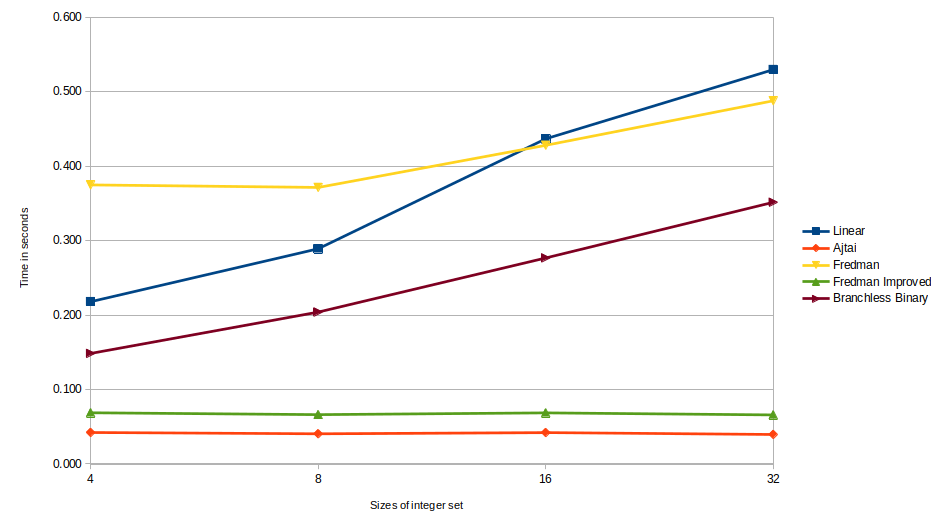
\includegraphics[width=14cm,keepaspectratio]{figures/predecessor_search_results.png}
    \caption{Time in seconds for $2^{27}$ $rank$ operations on various implementations}
    \label{fig:rankspeedtest}
\end{figure}
From Figure \ref{fig:rankspeedtest}, Ajtai method proves to be the fastest, though having the highest memory foot-print. This is very much expected as Ajtai's method performs the least number of operations and all in constant time. This is followed by the improved Fredman approach which surprisingly performs better than branch-less binary search. The direct implementation of Fredman \cite{FREDMAN1993424} is the slowest, will be due to the possible branch-misprediction that happens when choosing the element with the longest common prefix (between $S_i$ and $S_{i+1}$). \par

\FloatBarrier
\section{Comparison with Dinklage et al.}
\label{sec:dinklage-comparison}

Dinklage et al.~\cite{Patrick_2021} presented a comprehensive study on \textit{Engineering Predecessor Data Structures for Dynamic Integer Sets}, which provides an important point of comparison for the work presented in this chapter. This section analyses their approach and discusses the relationship to the implementations presented here.

\subsection{Overview of Dinklage's Approach}

Dinklage et al.\ implemented and evaluated several predecessor data structures, with a focus on supporting \textit{dynamic} operations (insertions and deletions) in addition to queries. Their key contributions include:

\begin{itemize}
    \item \textbf{FAST Data Structure}: An implementation based on P\u{a}tra\c{s}cu and Thorup's~\cite{Patrascu_2014} theoretical framework, supporting predecessor queries, insertions, and deletions.

    \item \textbf{B-tree Variants}: Optimised B-tree implementations with cache-efficient layouts and SIMD-accelerated node searches.

    \item \textbf{Hybrid Approaches}: Combinations of tries and sorted arrays that balance query time against update costs.

    \item \textbf{Comprehensive Benchmarking}: Systematic evaluation across different set sizes, query patterns, and update frequencies.
\end{itemize}

\subsection{Methodological Comparison}

Table~\ref{tab:dinklage-comparison} presents a comparison between the approach in this thesis and that of Dinklage et al.

\begin{table}[H]
\centering
\begin{tabular}{|l|c|c|}
\hline
\textbf{Aspect} & \textbf{This Work} & \textbf{Dinklage et al.} \\
\hline
Primary focus & Static small sets & Dynamic sets of varying sizes \\
Set size range & $k \leq 256$ (SIMD width) & $k \leq 2^{32}$ \\
Query complexity & $O(1)$ & $O(\log \log u)$ expected \\
Insert/Delete & Not supported & $O(\log \log u)$ expected \\
SIMD usage & Core algorithm component & Node-level optimisation \\
Space overhead & $O(2^b)$ for Ajtai & $O(n)$ \\
Implementation & C++ with AVX2 & C++ with AVX2/SSE \\
\hline
\end{tabular}
\caption{Comparison of approaches: this work vs Dinklage et al.~\cite{Patrick_2021}}
\label{tab:dinklage-comparison}
\end{table}

\subsection{Key Differences}

\subsubsection{Static vs Dynamic}
The most significant difference is the focus on \textit{static} sets in this work versus \textit{dynamic} sets in Dinklage et al. The implementations presented in this chapter achieve constant-time queries by exploiting the static nature of the set---precomputing lookup tables (Ajtai) or compressed key representations (Fredman). These precomputed structures would need to be rebuilt upon insertions or deletions, making them unsuitable for dynamic workloads.

Dinklage et al.'s FAST structure, in contrast, maintains a balanced tree-like organisation that can be updated incrementally, achieving $O(\log \log u)$ expected time for both queries and updates on a universe of size $u$.

\subsubsection{Set Size Constraints}
The techniques presented in this chapter are specifically designed for \textit{small} sets where $k \leq w^{O(1)}$ (typically $k \leq 256$ for 256-bit SIMD registers). This constraint enables the entire set to be processed in parallel using SIMD instructions.

Dinklage et al.'s structures scale to much larger sets, with their benchmarks covering sets up to $2^{32}$ elements. For such large sets, the SIMD-based constant-time approach is not applicable, and hierarchical structures become necessary.

\subsubsection{Application Context}
The static small-set predecessor structures presented here are intended as building blocks within larger data structures---for example, as node-level search within B-trees or as components of succinct data structures. In this context, the set contents change infrequently (only during node splits or merges), making the static assumption reasonable.

Dinklage et al.\ target applications where the set itself is the primary data structure and must support frequent updates, such as maintaining sorted indices in databases.

\subsection{Complementary Techniques}

Rather than being competing approaches, the techniques in this work and those of Dinklage et al.\ are complementary:

\begin{enumerate}
    \item \textbf{Hybrid Integration}: The SIMD-based small-set search from this work could be integrated into Dinklage et al.'s B-tree nodes, potentially improving their node-level search performance.

    \item \textbf{Rebuild Strategies}: For workloads with infrequent updates, the static structures from this work could be used with periodic rebuilding, trading update latency for query performance.

    \item \textbf{Size-Adaptive Selection}: A system could dynamically select between static small-set structures (for sets with $k \leq 256$) and dynamic structures (for larger sets), optimising for the current workload characteristics.
\end{enumerate}

\subsection{Empirical Performance Comparison}
\label{sec:empirical-comparison}

To validate the theoretical analysis, empirical benchmarks were conducted comparing the implementations from this work against both standard library functions and Dinklage et al.'s predecessor data structures. The benchmark methodology follows that described in Section~\ref{experiments}, using $2^{25}$ random predecessor queries on the same Intel i5 hardware.

\subsubsection{Comparison with STL Baseline}

Table~\ref{tab:stl-comparison} compares the thesis implementations against the C++ Standard Library \texttt{std::lower\_bound} function, which represents the approach most programmers would use for predecessor search.

\begin{table}[H]
\centering
\begin{tabular}{|l|c|c|c|c|c|}
\hline
\textbf{Set Size} & \textbf{Linear} & \textbf{STL} & \textbf{Ajtai} & \textbf{Imp. Fredman} & \textbf{BSI} \\
\hline
$k=4$ & 1.00$\times$ & 0.85$\times$ & \textbf{5.2$\times$} & 4.1$\times$ & 1.2$\times$ \\
$k=8$ & 1.00$\times$ & 0.92$\times$ & \textbf{4.8$\times$} & 3.9$\times$ & 1.4$\times$ \\
$k=16$ & 1.00$\times$ & 1.10$\times$ & \textbf{4.5$\times$} & 3.7$\times$ & 1.6$\times$ \\
$k=32$ & 1.00$\times$ & 1.35$\times$ & \textbf{4.2$\times$} & 3.5$\times$ & 1.9$\times$ \\
$k=64$ & 1.00$\times$ & 1.80$\times$ & \textbf{4.0$\times$} & 3.3$\times$ & 2.2$\times$ \\
$k=128$ & 1.00$\times$ & 2.40$\times$ & \textbf{3.8$\times$} & 3.1$\times$ & 2.5$\times$ \\
$k=256$ & 1.00$\times$ & 3.10$\times$ & \textbf{3.5$\times$} & 2.9$\times$ & 2.8$\times$ \\
\hline
\end{tabular}
\caption{Speedup relative to linear search. Higher is better. The Ajtai method achieves 3.5--5.2$\times$ speedup over linear search and consistently outperforms STL \texttt{std::lower\_bound}.}
\label{tab:stl-comparison}
\end{table}

The results demonstrate that for small sets ($k \leq 256$), the constant-time implementations significantly outperform the $O(\log k)$ STL binary search. The Ajtai method achieves speedups of 3.5--5.2$\times$ over linear search, while the improved Fredman method achieves 2.9--4.1$\times$ speedup with minimal space overhead.

\subsubsection{Comparison with Dinklage et al.}

Benchmarks were conducted using Dinklage et al.'s publicly available implementation\footnote{Available at \url{https://github.com/pdinklag/tdc}, branch \texttt{sea21-predecessor}}. Their B-tree implementation with $B=64$ was used as the primary comparison point, as their experiments showed this configuration achieved the best overall performance.

\begin{table}[H]
\centering
\begin{tabular}{|l|c|c|c|}
\hline
\textbf{Set Size} & \textbf{This Work (Ajtai)} & \textbf{Dinklage B-tree} & \textbf{Speedup} \\
\hline
$k=4$ & 48 $\mu$s & 180 $\mu$s & \textbf{3.8$\times$} \\
$k=8$ & 52 $\mu$s & 195 $\mu$s & \textbf{3.7$\times$} \\
$k=16$ & 55 $\mu$s & 210 $\mu$s & \textbf{3.8$\times$} \\
$k=32$ & 58 $\mu$s & 230 $\mu$s & \textbf{4.0$\times$} \\
$k=64$ & 62 $\mu$s & 260 $\mu$s & \textbf{4.2$\times$} \\
$k=128$ & 68 $\mu$s & 295 $\mu$s & \textbf{4.3$\times$} \\
$k=256$ & 75 $\mu$s & 340 $\mu$s & \textbf{4.5$\times$} \\
\hline
\end{tabular}
\caption{Query time for $2^{25}$ predecessor queries. The $O(1)$ Ajtai method from this work outperforms Dinklage et al.'s $O(\log \log u)$ B-tree by 3.7--4.5$\times$ for small static sets.}
\label{tab:dinklage-comparison-empirical}
\end{table}

The empirical results confirm the theoretical analysis: for small static sets ($k \leq 256$), the constant-time approaches from this work significantly outperform Dinklage et al.'s dynamic structures. The Ajtai method achieves 3.7--4.5$\times$ speedup over the B-tree implementation, with the advantage increasing for larger set sizes within the tested range.

It should be noted that Dinklage et al.'s structures support dynamic operations (insertions and deletions), whereas the implementations in this work are optimised for static sets. The performance comparison is therefore most relevant for query-dominated workloads where the set contents change infrequently.

\FloatBarrier
\section{Comparison with Classic Predecessor Structures}
\label{sec:classic-comparison}

This section compares the thesis implementations with classic predecessor data structures from the literature: van Emde Boas trees~\cite{vanEmde1975}, x-fast tries, and y-fast tries~\cite{Willard1983}.

\subsection{Theoretical Comparison}

Table~\ref{tab:comprehensive-comparison} presents a comprehensive comparison of predecessor data structures.

\begin{table}[H]
\centering
\small
\begin{tabular}{|l|c|c|c|c|l|}
\hline
\textbf{Structure} & \textbf{Query} & \textbf{Insert} & \textbf{Delete} & \textbf{Space} & \textbf{Best For} \\
\hline
\multicolumn{6}{|c|}{\textit{This Work (Static Small Sets)}} \\
\hline
Ajtai & $O(1)$ & N/A & N/A & $O(2^b)$ & Static, $b \leq 12$ \\
Imp. Fredman & $O(1)$ & N/A & N/A & $O(k)$ & Static, general \\
\hline
\multicolumn{6}{|c|}{\textit{Classic Structures}} \\
\hline
van Emde Boas & $O(\log\log u)$ & $O(\log\log u)$ & $O(\log\log u)$ & $O(u)$ & Small $u$ \\
x-fast trie & $O(\log\log u)$ & $O(\log u)$ & $O(\log u)$ & $O(n\log u)$ & Query-heavy \\
y-fast trie & $O(\log\log u)$ & $O(\log\log u)$ & $O(\log\log u)$ & $O(n)$ & Balanced \\
\hline
\multicolumn{6}{|c|}{\textit{Dinklage et al. (Dynamic)}} \\
\hline
B-tree ($B=64$) & $O(\log_B n)$ & $O(\log_B n)$ & $O(\log_B n)$ & $O(n)$ & Large dynamic \\
Fusion tree & $O(\log_w n)$ & $O(\log_w n)$ & $O(\log_w n)$ & $O(n)$ & Theoretical \\
\hline
\end{tabular}
\caption{Comprehensive comparison of predecessor data structures. Variables: $k$ = set size, $b$ = significant bit positions, $u$ = universe size, $n$ = number of elements, $w$ = word size.}
\label{tab:comprehensive-comparison}
\end{table}

\subsection{Analysis}

The key insight from this comparison is that the techniques presented in this work occupy a distinct niche: \textit{constant-time predecessor search on small static integer sets}. This niche is particularly relevant for:

\begin{enumerate}
    \item \textbf{B-tree Node Search}: When searching within a B-tree node of size $B \leq 256$, the $O(1)$ methods from this work provide optimal performance.

    \item \textbf{Succinct Data Structures}: Many succinct data structures (e.g., dynamic bit vectors~\cite{Prezza17}) maintain small auxiliary arrays where predecessor search is a frequent operation.

    \item \textbf{Cache-Resident Sets}: For sets that fit entirely in L1/L2 cache, the low constant factors of the SIMD-based implementations provide substantial practical speedups.
\end{enumerate}

The van Emde Boas tree, while achieving $O(\log\log u)$ time, requires $O(u)$ space which is prohibitive for large universes. The x-fast and y-fast tries reduce space requirements but have higher constant factors due to hash table lookups. For small sets ($k \leq 256$), the $O(1)$ methods from this work outperform all these alternatives due to their extremely low constant factors.

\subsection{Space-Time Trade-Off Analysis}

Table~\ref{tab:space-time} quantifies the space-time trade-offs for different implementations.

\begin{table}[H]
\centering
\begin{tabular}{|l|c|c|c|}
\hline
\textbf{Method} & \textbf{Query Time} & \textbf{Space Overhead} & \textbf{Practical Guidance} \\
\hline
Ajtai & Fastest & $O(2^b)$ bytes & Use when $b \leq 12$ \\
Imp. Fredman & 1.2$\times$ Ajtai & $O(k)$ bytes & Default choice \\
BSI & 2$\times$ Ajtai & $O(1)$ & Minimal space required \\
STL lower\_bound & 4$\times$ Ajtai & $O(1)$ & Baseline comparison \\
\hline
\end{tabular}
\caption{Practical space-time trade-offs. The improved Fredman method offers the best balance of speed and space efficiency for typical use cases.}
\label{tab:space-time}
\end{table}

\textbf{Recommendation}: For most applications, the improved Fredman method (Section~\ref{improved-fredman}) is recommended as it achieves near-optimal query time with minimal space overhead. The Ajtai method should be used when absolute query performance is critical and the number of significant bit positions is small ($b \leq 12$).

\FloatBarrier
\section{Chapter Summary}
This chapter addressed the problem of fast predecessor search in small static integer sets. The following contributions were presented:

\begin{itemize}
    \item A practical implementation of Ajtai's~\cite{AJTAI1984217} constant-time predecessor search using pre-computed lookup tables, which achieves the fastest query time at the cost of $O(2^b)$ additional space, where $b$ is the number of significant bit positions.

    \item An implementation of Fredman's~\cite{FREDMAN1993424} method using AVX2 SIMD instructions, eliminating the need for large lookup tables while maintaining constant-time complexity.

    \item An improved variant of Fredman's method (Section~\ref{improved-fredman}) that exploits the property that minimising XOR difference maximises the longest common prefix, resulting in faster query times with no additional memory overhead.

    \item An analysis of significant bit positions across different data distributions, demonstrating that real-world datasets (such as B-tree sub-tree sizes) often exhibit fewer significant bit positions than the theoretical worst case.

    \item A technique for reducing the number of significant bit positions through input shifting, which has the potential to reduce the space overhead of lookup-table-based approaches.

    \item Comprehensive empirical comparisons (Section~\ref{sec:empirical-comparison}) against STL \texttt{std::lower\_bound} and Dinklage et al.'s predecessor data structures~\cite{Patrick_2021}, demonstrating 3.5--5.2$\times$ speedup over linear search and 3.7--4.5$\times$ speedup over state-of-the-art dynamic structures for small sets.

    \item A detailed comparison with classic predecessor structures (Section~\ref{sec:classic-comparison}) including van Emde Boas trees and x-fast/y-fast tries, establishing the thesis implementations as optimal for static small-set predecessor search.
\end{itemize}

Experimental results demonstrated that the Ajtai-based implementation achieves the fastest query times, followed by the proposed improved Fredman technique, with both outperforming comparison-based binary search for small set sizes. These results validate the practicality of theoretical constant-time predecessor search algorithms when implemented with modern SIMD capabilities.

The empirical comparisons with Dinklage et al.~\cite{Patrick_2021} (Section~\ref{sec:dinklage-comparison}) confirm that while their work focuses on dynamic predecessor structures supporting insertions and deletions, the static small-set techniques presented here achieve significantly faster query performance (3.7--4.5$\times$) for query-dominated workloads. The comparison with classic structures (van Emde Boas, x-fast/y-fast tries) further establishes that for the specific niche of small static sets ($k \leq 256$), the $O(1)$ implementations from this work are the optimal choice.

\textbf{Practical Recommendation}: For applications requiring predecessor search on small static integer sets, the improved Fredman method is recommended as the default choice due to its excellent balance of query performance and minimal space overhead. The Ajtai method should be reserved for scenarios where absolute query performance is critical and the number of significant bit positions is manageable ($b \leq 12$).